%!TEX root = doc.tex
\section{\apiname{} Architecture} % (fold)
\label{sec:proposal}

The software described in this paper is the result of a need to convert certain agent-based applications written for JADE or Repast from one framework to the other. This is also the reasoning behind our decision to base our implementation on JADE's. In this section we try to give a thorough description of \apiname{}'s architecture while comparing our design decisions with those of JADE.

JADE's approach consists of using behaviors for the agents that take the role of initiator or responder and provide essential functionality of each protocol, allowing the programmer to implement his own handlers for the messages while maintaining all the communication logic behind the scenes. This architecture allows the programmer to focus on the specifics of the application without having to deal with the implementation of the protocols and the development of the network infrastructure. \cite{bellifemine2003jade}

\apiname{}'s implementation of the FIPA interaction protocols is essentially based on JADE. However, conceptual adaptations had to be made to incorporate the concept of time in JADE's protocols, which are asynchronous and event-driven. In \apiname{}, communication happens asynchronously but not event-driven. As Figure \ref{fig:com-example} shows, agent execution in Repast in not concurrent. Repast grants execution rights to each agent's tasks until they finish, in no particular order.

\begin{figure}[h]
	\centering
	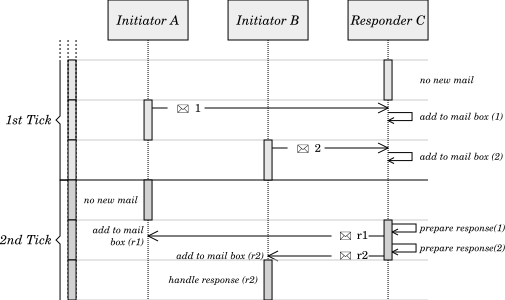
\includegraphics[width=0.5\textwidth]{figures/tickExample.png}
	\caption[Communication example]{
		Communication example in a single tick.
		This is a best case scenario where the order of execution of
		the agents by Repast was favorable to communication. It's not
		unexpected for Agents A and B to execute again once before
		Agent C does.
	}
	\label{fig:com-example}
\end{figure}



Figure \ref{fig:arch} illustrates the details of \apiname{}'s architecture. Most concepts represented in this diagram are present in JADE, namely the Agent, ACL Message, Behavior, MTS and DF service.

An agent in \apiname{} contains a queue of Behaviors and a mail box. On each ``round'', these behaviors are schedules to be executed and some will take care of handling the messages arrived at the mail box.

The protocol package contains the implementation of different FIPA protocols. The ones ported from JADE were the ``Request-like'' Achieve RE, Propose and Contract Net. Other protocols can be created by extending these and creating new behaviors can be done by extending the main Behavior.

Analogous to JADE, the DF service in \apiname{} allows an agent to find other agents. It is possible to filter the agent search by service, i.e. specify what behaviors or protocols they should be executing. The MTS is a facility used for message delivery.


\begin{figure}[h]
	\centering
	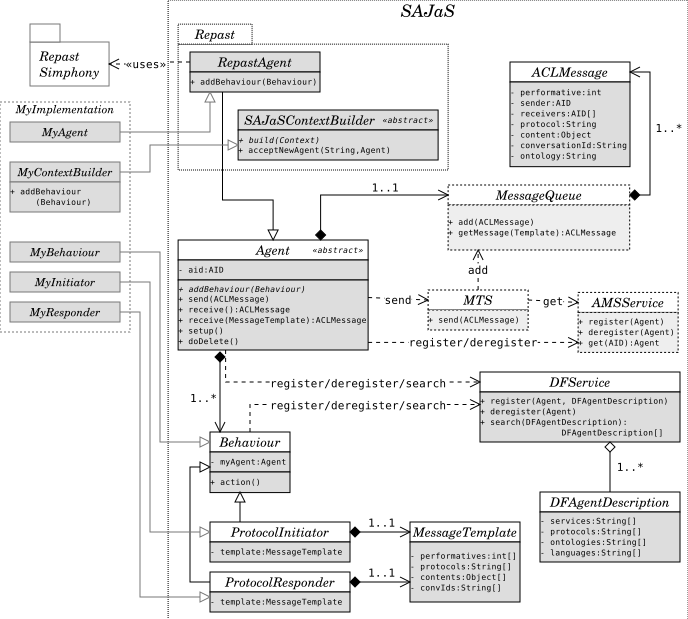
\includegraphics[width=0.5\textwidth]{figures/repacl_arch.png}
	\caption{Detailed architecture or \apiname{}}
	\label{fig:arch}
\end{figure}

% section proposal (end)